\part{Transformers}
\title{Transformers}  
\date{}  
\frame{\titlepage} 

%%%%%%%%%%%%%%%%%%%%%%%%%%%%%%%%%%%%%%%%%%%%%%%%%%%%%%%%%%%%%
%% Transformer definition %%
%%%%%%%%%%%%%%%%%%%%%%%%%%%%%%%%%%%%%%%%%%%%%%%%%%%%%%%%%%%%%
\begin{frame}
	\frametitle{Transformer definition}
    \begin{columns}
		\begin{column}{0.65\textwidth}
            \begin{varblock}{Transformer}
                A transformer is a static device that transfers electrical energy between two or more circuits through electromagnetic induction. It converts the AC voltage levels between inputs and outputs.   
            \end{varblock}
            \begin{itemize}
                \item While a transformer is sometimes called a ``static~machine'', it does not meet the formal definition of an electrical machine (compare first chapter).
                \item However, transformers share some working principles with electrical machines and are also often used as components of electrical power systems including drives.
            \end{itemize}
		\end{column}
        \hfill
		\begin{column}{0.35\textwidth}
			\begin{figure}
				\centering
				\includegraphics[width=0.75\textwidth]{fig/lec04/Transformer_rural_pole.jpg}
				\caption{Transformer integrated at a utility pole (source: \href{https://pxhere.com/en/photo/795672}{pxhere.com}, public domain)}
			\end{figure}
		\end{column}
		\end{columns}
\end{frame}

%%%%%%%%%%%%%%%%%%%%%%%%%%%%%%%%%%%%%%%%%%%%%%%%%%%%%%%%%%%%%
%% Examples of transformers %%
%%%%%%%%%%%%%%%%%%%%%%%%%%%%%%%%%%%%%%%%%%%%%%%%%%%%%%%%%%%%%
\begin{frame}
	\frametitle{Examples of transformers}
	\begin{figure}
		\centering
		\begin{subfigure}[b]{0.49\textwidth}
			\centering
			\includegraphics[width=0.45\textwidth]{fig/lec04/Power_supply_transformer.jpg}
			\caption{Power supply transformer (source: \href{https://commons.wikimedia.org/wiki/File:Philips_N4422_-_power_supply_transformer-2098.jpg}{Wikimedia Commons}, R.~Spekking, \href{https://creativecommons.org/licenses/by-sa/4.0/deed}{CC BY-SA 4.0})}
		\end{subfigure}
		\hfill
		\begin{subfigure}[b]{0.49\textwidth}
			\centering
			\includegraphics[width=0.45\textwidth]{fig/lec04/Single_phase_transformer.jpg}
			\caption{Single-phase transformer (source: \href{https://commons.wikimedia.org/wiki/File:DB_Unterwerk_Güsen,_Trafo_p.jpg}{Wikimedia Commons}, Georg, \href{https://creativecommons.org/licenses/by-sa/4.0/deed.en}{CC BY-SA 4.0})}
		\end{subfigure}
		\\
		\begin{subfigure}[b]{0.49\textwidth}
			\centering
			\includegraphics[width=0.45\textwidth]{fig/lec04/Three_phase_transformer.jpg}
			\caption{Three-phase transformer (source: \href{https://commons.wikimedia.org/wiki/File:Dornbirn-Umspannwerk_Werben-110kV_FS6-Anlage_Trafo_Elin_220-110kV-01ASD.jpg}{Wikimedia Commons}, Asurnipal, \href{https://creativecommons.org/licenses/by-sa/4.0/deed.en}{CC BY-SA 4.0})}
		\end{subfigure}
		\hfill
		\begin{subfigure}[b]{0.49\textwidth}
			\centering
			\includegraphics[width=0.45\textwidth]{fig/lec04/Tapped_transformer.jpg}
			\caption{Variable tapped transformer (source: \href{https://commons.wikimedia.org/wiki/File:Variable-tap_regulating_transformer_(Rankin_Kennedy,_Electrical_Installations,_Vol_II,_1909).jpg}{Wikimedia Commons}, public domain)}
		\end{subfigure}
		\caption*{Examples of transformers} 
        \label{fig:examples_transformers}
	\end{figure}
\end{frame}

%%%%%%%%%%%%%%%%%%%%%%%%%%%%%%%%%%%%%%%%%%%%%%%%%%%%%%%%%%%%%
%% Electromagnetic modeling of the single-phase transformer %%
%%%%%%%%%%%%%%%%%%%%%%%%%%%%%%%%%%%%%%%%%%%%%%%%%%%%%%%%%%%%%
\begin{frame}
	\frametitle{Electromagnetic modeling of the single-phase transformer}
    \begin{columns}
		\begin{column}{0.45\textwidth}
            Recap from \eqref{eq:flux_linkage_matrix_transformer}: for some given current $\bm{i}$, the flux linkages $\bm{\psi}$ in the transformer windings are
			\begin{equation*}
				\bm{\psi} = \begin{bmatrix} \psi_1 \\ \psi_2 \end{bmatrix} = \begin{bmatrix} L_1 & M \\ M & L_2 \end{bmatrix} \begin{bmatrix} i_1 \\ i_2 \end{bmatrix} = \bm{L}\bm{i}
			\end{equation*}
			where $L_1$ and $L_2$ are the self-inductances of the primary and secondary winding, respectively, and $M$ is the mutual inductance.
			\\[1em]
			Note: The above equation is an algebraic relation, that is, it is valid for any time instant $t$ and applies to both AC and DC excitation of the transformer. 
		\end{column}
        \hfill
		\begin{column}{0.525\textwidth}
			\begin{figure}
				\centering
				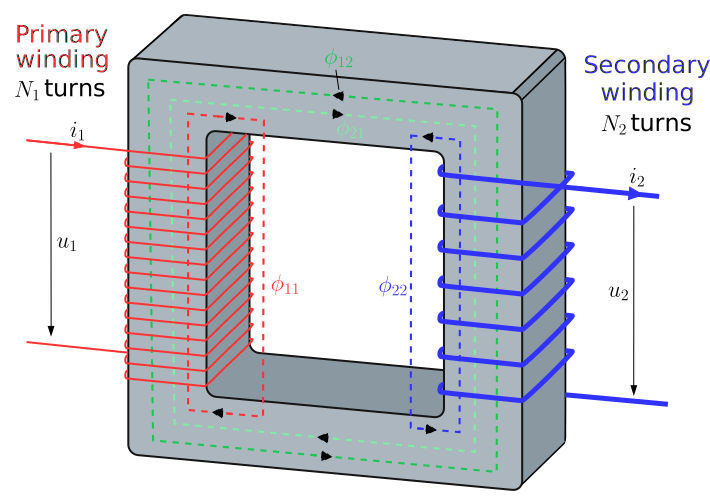
\includegraphics[height=0.575\textheight]{fig/lec02/Transformer3d_col3.pdf}
			\end{figure}
		\end{column}
		\end{columns}
\end{frame}

%%%%%%%%%%%%%%%%%%%%%%%%%%%%%%%%%%%%%%%%%%%%%%%%%%%%%%%%%%%%%
%% Electromagnetic modeling of the single-phase transformer (cont.) %%
%%%%%%%%%%%%%%%%%%%%%%%%%%%%%%%%%%%%%%%%%%%%%%%%%%%%%%%%%%%%%
\begin{frame}
	\frametitle{Electromagnetic modeling of the single-phase transformer (cont.)}
		The dynamic transformer behavior can be represented by the ECD in \figref{fig:General_transformer_ECD}, which also considers the internal resistances of the windings. Applying Faraday's law, the resulting differential equations are:
		\begin{align}
			u_1(t) = R_1 i_1(t) + \frac{\mathrm{d}\psi_1(t)}{\mathrm{d}t}, \qquad u_2(t) = R_2 i_2(t) + \frac{\mathrm{d}\psi_2(t)}{\mathrm{d}t}. \label{eq:transformer_differential_equations}
		\end{align}
		Inserting \eqref{eq:flux_linkage_matrix_transformer} delivers:
		\begin{align}
			u_1(t) = R_1 i_1(t) + L_1 \frac{\mathrm{d}i_1(t)}{\mathrm{d}t} + M \frac{\mathrm{d}i_2(t)}{\mathrm{d}t}, \qquad
			u_2(t) = R_2 i_2(t) + L_2 \frac{\mathrm{d}i_2(t)}{\mathrm{d}t} + M \frac{\mathrm{d}i_1(t)}{\mathrm{d}t}. \label{eq:transformer_differential_equations_2}
		\end{align}
		
\begin{figure}
\begin{columns}
	\begin{column}{0.55\textwidth}
            \centering
            
\includegraphics[width=0.8\textwidth]{fig/lec04/General_transformer_ECD.pdf}
    \end{column}
    \begin{column}{0.45\textwidth}
        \caption{\raggedright General equivalent circuit diagram (ECD) of a transformer (note: that both ports of the transformer are denoted in the load convention reference frame which is an arbitrary representation decision).}
		\label{fig:General_transformer_ECD}
    \end{column}
\end{columns}
\end{figure}
\end{frame}

%%%%%%%%%%%%%%%%%%%%%%%%%%%%%%%%%%%%%%%%%%%%%%%%%%%%%%%%%%%%%
%% Electromagnetic modeling of the single-phase transformer (cont.) %%
%%%%%%%%%%%%%%%%%%%%%%%%%%%%%%%%%%%%%%%%%%%%%%%%%%%%%%%%%%%%%
\begin{frame}
	\frametitle{Electromagnetic modeling of the single-phase transformer (cont.)}
		The \eqref{eq:transformer_differential_equations_2} can be represented by the T-type ECD in \figref{fig:Transformer_T_ECD}. It may be noted that $L_1-M$ and $L_2-M$ can have negative values due to the model representation. 
		\\[1em]
		By rearranging and substituting, we can also obtain the state-space representation of the transformer from \eqref{eq:transformer_differential_equations_2} by utilizing the leakage coefficient $\sigma = 1- k^2 = 1 - M^2/(L_1 L_2)$:
		\begin{equation}
			\renewcommand*{\arraystretch}{1.4}
			\frac{\mathrm{d}}{\mathrm{d}t}\begin{bmatrix}i_1(t)\\i_2(t)\end{bmatrix}=\frac{\mathrm{d}}{\mathrm{d}t}\bm{i}(t) = \begin{bmatrix} - \frac{R_1}{\sigma L_1} & \frac{R_2 M}{\sigma L_1 L_2}\\  \frac{R_1 M}{\sigma L_1 L_2} & -\frac{R_2}{\sigma L_2} \end{bmatrix} \bm{i}(t) + \begin{bmatrix} \frac{1}{\sigma L_1} & -\frac{M}{\sigma L_1 L_2} \\ -\frac{M}{\sigma L_1 L_2} & \frac{1}{\sigma L_2} \end{bmatrix} \bm{u}(t).
		\end{equation}

\begin{figure}
\begin{columns}
	\begin{column}{0.55\textwidth}
            \centering
            
\includegraphics[width=0.9\textwidth]{fig/lec04/Transformer_T_ECD.pdf}
    \end{column}
    \begin{column}{0.45\textwidth}
        \caption{\raggedright T-type ECD of a transformer}
		\label{fig:Transformer_T_ECD}
    \end{column}
\end{columns}
\end{figure}
\end{frame}